%
\documentclass{chi-ext}
% Please be sure that you have the dependencies (i.e., additional LaTeX packages) to compile this example.
% See http://personales.upv.es/luileito/chiext/

%% EXAMPLE BEGIN -- HOW TO OVERRIDE THE DEFAULT COPYRIGHT STRIP -- (July 22, 2013 - Paul Baumann)
% \copyrightinfo{Permission to make digital or hard copies of all or part of this work for personal or classroom use is granted without fee provided that copies are not made or distributed for profit or commercial advantage and that copies bear this notice and the full citation on the first page. Copyrights for components of this work owned by others than ACM must be honored. Abstracting with credit is permitted. To copy otherwise, or republish, to post on servers or to redistribute to lists, requires prior specific permission and/or a fee. Request permissions from permissions@acm.org. \\
% {\emph{CHI'14}}, April 26--May 1, 2014, Toronto, Canada. \\
% Copyright \copyright~2014 ACM ISBN/14/04...\$15.00. \\
% DOI string from ACM form confirmation}
%% EXAMPLE END -- HOW TO OVERRIDE THE DEFAULT COPYRIGHT STRIP -- (July 22, 2013 - Paul Baumann)

\title{Firmware: The Missing Blueprint}

% Notice how author names are alternately typesetted to appear ordered in 2-column format;
% i.e., the first 4 autors on the first column and the other 4 auhors on the second column.
% Actually, it's up to you to strictly adhere to this author notation.
\author{
  \alignauthor{
        \textbf{Cefn Hoile}\\
        \affaddr{AuthorCo, Inc.}\\
        \affaddr{123 Author Ave.}\\
        \affaddr{Authortown, PA 54321 USA}\\
        \email{author1@anotherco.com}
  }
  \vspace{2em}
  \begin{figure}
  \centering
  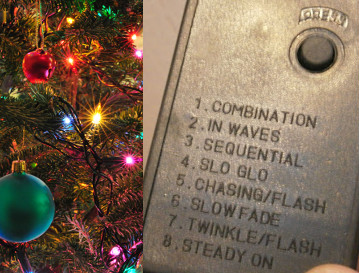
\includegraphics[width=250]{sample.jpg}
  \end{figure}
  \vspace{2em}
}

% Paper metadata (use plain text, for PDF inclusion and later re-using, if desired)
\def\plaintitle{CHI LaTeX Extended Abstracts Template}
\def\plainauthor{Luis A. Leiva}
\def\plainkeywords{Guides, instructions, author's kit, conference publications}
\def\plaingeneralterms{Documentation, Standardization}

\hypersetup{
  % Your metadata go here
  pdftitle={\plaintitle},
  pdfauthor={\plainauthor},  
  pdfkeywords={\plainkeywords},
  pdfsubject={\plaingeneralterms},
  % Quick access to color overriding:
  %citecolor=black,
  %linkcolor=black,
  %menucolor=black,
  %urlcolor=black,
}

\usepackage{graphicx}   % for EPS use the graphics package instead
\usepackage{balance}    % useful for balancing the last columns
\usepackage{bibspacing} % save vertical space in references
\renewcommand{\sfdefault}{phv} % Arial
\fontsize{8.5}{10}
\begin{document}

\marginpar{
\begin{figure}
  \begin{center}
  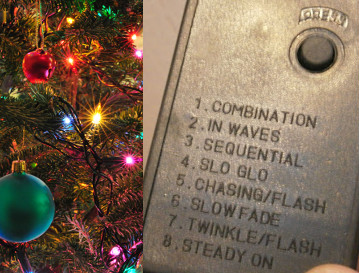
\includegraphics[width=\marginparwidth]{sample.jpg}
  \caption{A marginal figure.}
  \label{fig:marginparsample}
  \end{center}  
\end{figure}
}

\marginpar{
\begin{figure}
  \begin{center}
  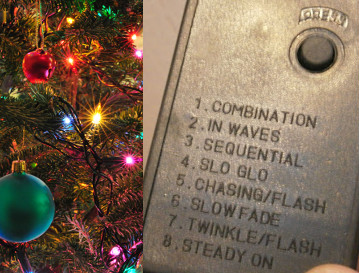
\includegraphics[width=\marginparwidth]{sample.jpg}
  \caption{A marginal figure.}
  \label{fig:marginparsample}
  \end{center}  
\end{figure}
}

\marginpar{
\begin{figure}
  \begin{center}
  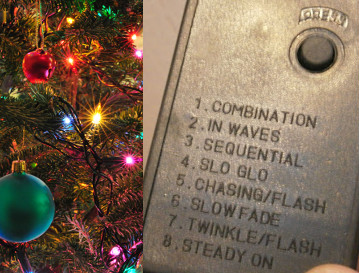
\includegraphics[width=\marginparwidth]{sample.jpg}
  \caption{A marginal figure.}
  \label{fig:marginparsample}
  \end{center}  
\end{figure}
}

\marginpar{
\begin{figure}
  \begin{center}
  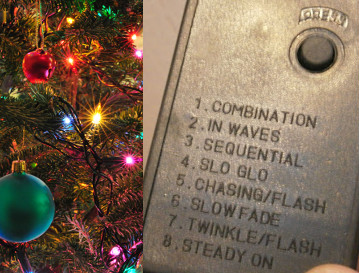
\includegraphics[width=\marginparwidth]{sample.jpg}
  \caption{A marginal figure.}
  \label{fig:marginparsample}
  \end{center}  
\end{figure}
}
\maketitle

\begin{abstract}
In the process of realising a product, choices must be made about its configuration. For a digitally-controlled product, its programmed behaviour, or firmware, is an element which will heavily influence user experience. We contrast three caricatures of practice, where preferred product configurations  are either \emph{discovered}, \emph{decided} or \emph{designed}. On this analysis, established practice for selecting programmed behaviour does not satisfy the criteria for being \emph{designed}. We examine what obstacles exist to applying design practices when selecting product behaviour, and propose a programme to identify artefacts and processes which can facilitate this work.
\end{abstract}

\keywords{\plainkeywords}
\textcolor{red}{Mandatory section to be included in your final version.}

\category{H.5.m}{Information interfaces and presentation (e.g., HCI)}{Miscellaneous}. 
%See \cite{ACMCCS} 
See: \url{http://www.acm.org/about/class/1998/} 
for help using the ACM Classification system.
\textcolor{red}{Mandatory section to be included in your final version.}

\terms{\plaingeneralterms}
\textcolor{red}{Optional section to be included in your final version.}

\marginpar{
\begin{figure}
  \begin{center}
  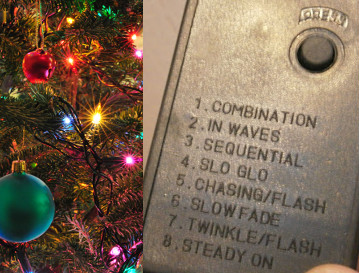
\includegraphics[width=\marginparwidth]{sample.jpg}
  \caption{A marginal figure.}
  \label{fig:marginparsample}
  \end{center}  
\end{figure}
}

\marginpar{
\begin{figure}
  \begin{center}
  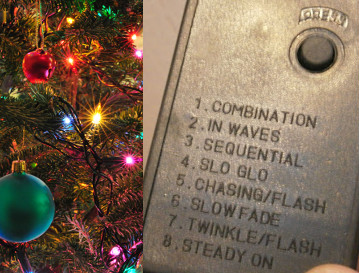
\includegraphics[width=\marginparwidth]{sample.jpg}
  \caption{A marginal figure.}
  \label{fig:marginparsample}
  \end{center}  
\end{figure}
}
\marginpar{
\begin{figure}
  \begin{center}
  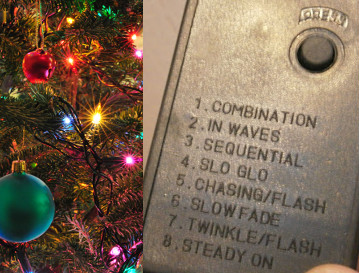
\includegraphics[width=\marginparwidth]{sample.jpg}
  \caption{A marginal figure.}
  \label{fig:marginparsample}
  \end{center}  
\end{figure}
}

\marginpar{
\begin{figure}
  \begin{center}
  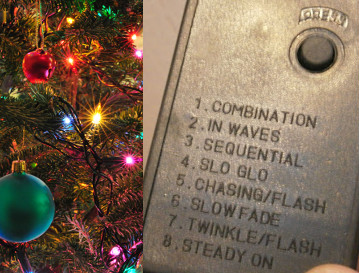
\includegraphics[width=\marginparwidth]{sample.jpg}
  \caption{A marginal figure.}
  \label{fig:marginparsample}
  \end{center}  
\end{figure}
}

% =============================================================================
\section{Introduction}
% =============================================================================

A broad, inclusive definition of design, is offered by Feng and Feenberg [], "a process of consciously shaping an artifact to adapt it to specific goals and environments". 
However, not all shaping practices adopt the same world-view. Some practices are modelled on the scientific method, and shaping choices are \emph{discovered}, by establishing facts, from which choices can be deduced. For example,  a material's physical properties can eliminate it from consideration, or experimental results in human perception can recommend employing a particular visual cue for users over an alternative. Within other practices there is a focus on mapping a space of solutions from which the preferred one will be \emph{decided} based on an implicit or explicit scheme of values and preference [].

In this paper, we reserve the phrase \emph{designed} for preferences which are arrived at through reflective processes [Schon] such as sketching [Brock and Craft] and bricolage [Levi-Strauss], building on design theorist's claims that sketching is "the archetypal activity of the design approach" [Fallman] and that "design in all its guises is a form of bricolage"[Louridas].

In a reflective process, preferences are neither \emph{discovered} through evidence gathering, nor \emph{decided} through systematic analysis of a space of configurations. Instead, the designer engages in a "conversation with materials" [Schon] resonating  "As designers conceive of a new idea or refine the details of an existing idea, the materials they use begin to 'talk back'" [Ozenc et al] [Brock and Craft

Co-design or design briefing

Architecture, blueprints and patterns.

% =============================================================================
\section{Sketches and Blueprints}
% =============================================================================
Informal and formal drawings are in use throughout the design process in fashion, architecture and product design, but no analog seems to exist for interactive behaviours. Sketches and blueprints of physical designs capture implementation commitments, guiding and constraining a specialist production process. However, they also stimulate and facilitate engagement with others without demanding they themselves have the skills to materialise the design. By contrast, in a firmware design process, the representations which characterise implementation commitments for code are accessible principally to programmers - those skilled in materialising digital behaviours - and can not effectively catalyse knowledge exchange with others. By excluding key stakeholders until working systems are ready to be tested, this restricts the design contributions they can make, and limits the potential for design thinking. In this paper, we explore behaviour blueprints as a design fiction and a rhetorical object. We outline the preferred features by analogy with effective tools from other disciplines, and we detail a program of future co-design experimentation which we hope will allow us to explore and validate candidate representations.

% =============================================================================
\section{Boundary Objects and Bricolage}
% =============================================================================
Please use an 8.5-point Verdana font, or other sans serifs font as close as possible in appearance to Verdana in {Use footnotes sparingly, if at all.}
As stated in the footnote, footnotes should rarely be used.

\marginpar{
\begin{figure}
  \begin{center}
  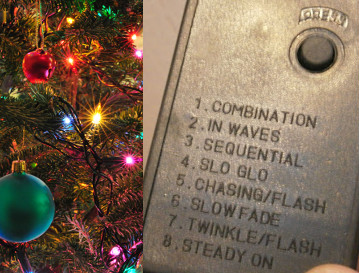
\includegraphics[width=\marginparwidth]{sample.jpg}
  \caption{A marginal figure.}
  \label{fig:marginparsample}
  \end{center}  
\end{figure}
}

\marginpar{
\begin{figure}
  \begin{center}
  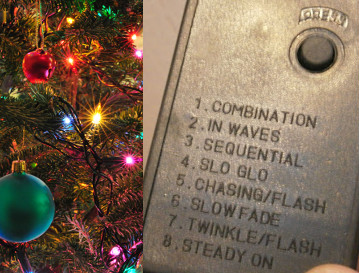
\includegraphics[width=\marginparwidth]{sample.jpg}
  \caption{A marginal figure.}
  \label{fig:marginparsample}
  \end{center}  
\end{figure}
}
\marginpar{
\begin{figure}
  \begin{center}
  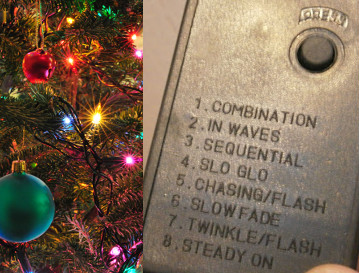
\includegraphics[width=\marginparwidth]{sample.jpg}
  \caption{A marginal figure.}
  \label{fig:marginparsample}
  \end{center}  
\end{figure}
}

\marginpar{
\begin{figure}
  \begin{center}
  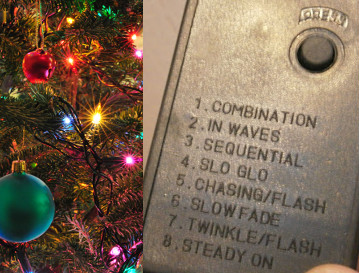
\includegraphics[width=\marginparwidth]{sample.jpg}
  \caption{A marginal figure.}
  \label{fig:marginparsample}
  \end{center}  
\end{figure}
}

\subsection{Language, style, and content}
% -----------------------------------------------------------------------------
The written and spoken language of SIGCHI is English. 
Spelling and punctuation may use any dialect of English (e.g., British, Canadian, US, etc.) provided this is done consistently. 
Hyphenation is optional. 
To ensure suitability for an international audience, please pay attention to the following:

\begin{itemize}\compresslist
\item   
Write in a straightforward style. 
Use simple sentence structure. 
Try to avoid long sentences and complex sentence structures. 
Use semicolons carefully.
\item   
Use common and basic vocabulary (e.g., use the word ``unusual" rather than the word ``arcane").
\item   
Briefly define or explain all technical terms. 
The terminology common to your practice/discipline may be different in other design practices/disciplines.
\item   
Spell out all acronyms the first time they are used in your text. 
For example, ``World Wide Web (WWW)".
\item   
Explain local references (e.g., not everyone knows all city names in a particular country).
\item   
Explain ``insidecalcr" comments. 
Ensure that your whole audience understands any reference whose meaning you do not describe (e.g., do not assume that everyone has used a Macintosh or a particular application).
\item   
Explain colloquial language and puns. 
Understanding phrases like ``red herring" requires a cultural knowledge of English. 
Humor and irony are difficult to translate.
\item   
Use unambiguous forms for culturally localized concepts, such as times, dates, currencies and numbers (e.g., ``1-5-97" or ``5/1/97" may mean 5 January or 1 May, and ``seven o'clock" may mean 7:00 am or 19:00).
\item   
Be careful with the use of gender-specific pronouns (he, she) and other gender-specific words (chairman, manpower, man-months). 
Use inclusive language (e.g., she or he, they, chair, staff, staff-hours, person-years) that is gender-neutral. 
If necessary, you may be able to use ``he" and ``she" in alternating sentences, so that the two genders occur equally often~\cite{Schwartz95}. 
\end{itemize}


% =============================================================================
\section{Figures}
% =============================================================================
The examples on this and following pages should help you get a feel for how screen-shots and other figures should be placed in the template. 
Be sure to make images large enough so the important details are legible and clear.



\begin{figure}
  \centering
  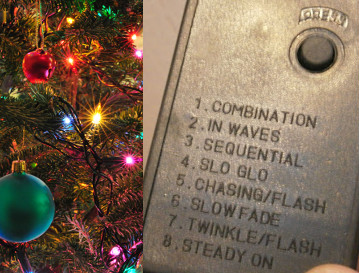
\includegraphics[width=\linewidth]{sample.jpg}
  \caption{Flashing Christmas Lights}
  \label{fig:sample}
\end{figure}

Your document may use color figures, which are included in the page limit; the figures must be usable when printed in black and white.
You can use the \LaTeX's \texttt{marginpar} command to insert figures in the (right) margin side of the document (see \autoref{fig:marginparsample}).

\marginpar{
\begin{figure}
  \begin{center}
  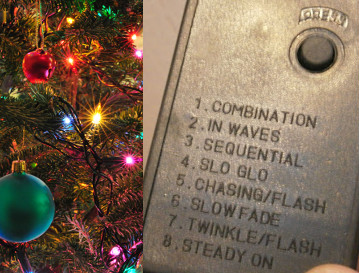
\includegraphics[width=\marginparwidth]{sample.jpg}
  \caption{A marginal figure.}
  \label{fig:marginparsample}
  \end{center}  
\end{figure}
}

\marginpar{
\begin{figure}
  \begin{center}
  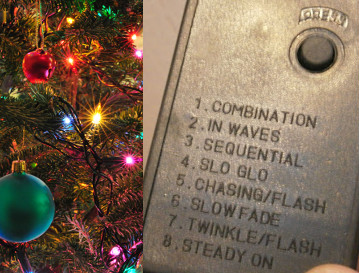
\includegraphics[width=\marginparwidth]{sample.jpg}
  \caption{A marginal figure.}
  \label{fig:marginparsample}
  \end{center}  
\end{figure}
}
\marginpar{
\begin{figure}
  \begin{center}
  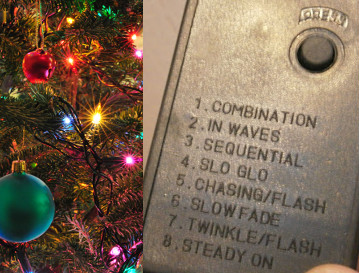
\includegraphics[width=\marginparwidth]{sample.jpg}
  \caption{A marginal figure.}
  \label{fig:marginparsample}
  \end{center}  
\end{figure}
}

\marginpar{
\begin{figure}
  \begin{center}
  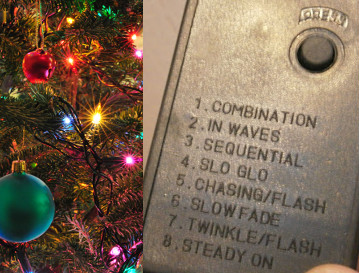
\includegraphics[width=\marginparwidth]{sample.jpg}
  \caption{A marginal figure.}
  \label{fig:marginparsample}
  \end{center}  
\end{figure}
}

% =============================================================================
\section{References and Citations}
% =============================================================================
Use a numbered list of references at the end of the article, ordered alphabetically by first author, and referenced by numbers in brackets \cite{Anderson92,Klemmer02,Mather00,Zellweger01}
For papers from conference proceedings, include the title of the paper and an abbreviated name of the conference (e.g., for Interact 2003 proceedings, use Proc. Interact 2003). 
Do not include the location of the conference or the exact date; do include the page numbers if available. 
See the examples of citations at the end of this document. 

Your references should be published materials accessible to the public.  
Internal technical reports may be cited only if they are easily accessible (i.e., you provide the address for obtaining the report within your citation) and may be obtained by any reader for a nominal fee.  
Proprietary information may not be cited. 
Private communications should be acknowledged in the main text, not referenced  (e.g., [Robertson, personal communication]).

% =============================================================================
\section{Accessibility}
% =============================================================================
The Executive Council of SIGCHI has committed to making SIGCHI conferences more inclusive for researchers, practitioners, and educators with disabilities. As a part of this goal, the all authors are asked to work on improving the accessibility of their submissions. Specifically, we encourage authors to carry out the following five steps:
\begin{enumerate}
        \item Add alternative text to all figures
        \item Mark table headings
        \item Add tags to the PDF
        \item Verify the default language
        \item Set the tab order to ``Use Document Structure''
\end{enumerate}
Unfortunately good tools do not yet exist to create tagged PDF files from Latex. LaTeX users will need to carry out all of the above steps in the PDF directly using Adobe Acrobat, after the PDF has been generated.
 
For more information and links to instructions and resources, please see:
{\url{http://chi2014.acm.org/authors/guide-to-an-accessible-submission}}.

% =============================================================================
\section{Producing and testing PDF files}
% =============================================================================
We recommend that you produce a PDF version of your submission well before the final deadline. 
Besides making sure that you are able to produce a PDF, you will need to check that (a) the length of the file remains within the submission category's page limit, (b) the PDF file size is 4 megabytes or less, and (c) the file can be read and printed using Adobe Acrobat Reader. 
Test your PDF file by viewing or printing it with the same software we will use when we receive it, Adobe Acrobat Reader Version 7. 
This is widely available at no cost from~\cite{Acrobat7}.  
Note that most reviewers will use a North American/European version of Acrobat reader, which cannot handle documents containing non-North American or non-European fonts (e.g. Asian fonts).  
Please therefore do not use Asian fonts, and verify this by testing with a North American/European Acrobat reader (obtainable as above). Something as minor as including a space or punctuation character in a two-byte font can render a file unreadable.

\marginpar{
\begin{figure}
  \begin{center}
  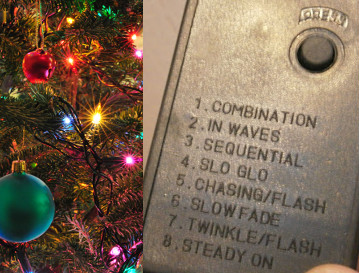
\includegraphics[width=\marginparwidth]{sample.jpg}
  \caption{A marginal figure.}
  \label{fig:marginparsample}
  \end{center}  
\end{figure}
}

\marginpar{
\begin{figure}
  \begin{center}
  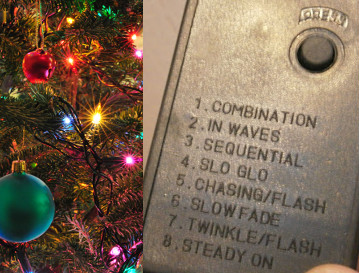
\includegraphics[width=\marginparwidth]{sample.jpg}
  \caption{A marginal figure.}
  \label{fig:marginparsample}
  \end{center}  
\end{figure}
}

\marginpar{
\begin{figure}
  \begin{center}
  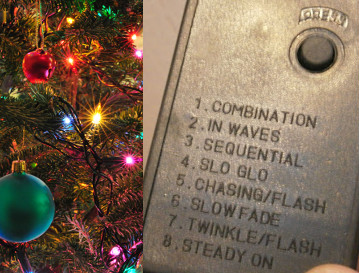
\includegraphics[width=\marginparwidth]{sample.jpg}
  \caption{A marginal figure.}
  \label{fig:marginparsample}
  \end{center}  
\end{figure}
}

\marginpar{
\begin{figure}
  \begin{center}
  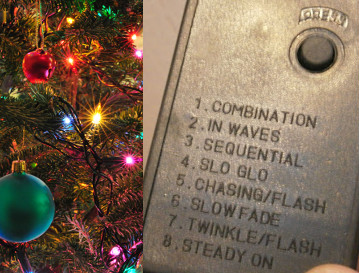
\includegraphics[width=\marginparwidth]{sample.jpg}
  \caption{A marginal figure.}
  \label{fig:marginparsample}
  \end{center}  
\end{figure}
}

% =============================================================================
\section{Dummy text}
% =============================================================================
Lorem ipsum dolor sit amet, consectetur adipiscing elit. Duis ut eros semper lectus vehicula elementum. Vestibulum ante ipsum primis in faucibus orci luctus et ultrices posuere cubilia Curae; Aliquam quis mi sapien. Suspendisse potenti. Mauris ultrices euismod velit sed dictum. Nullam auctor, nulla tincidunt dapibus suscipit, velit leo convallis metus, vel commodo libero erat in dolor. In laoreet porttitor ligula, porta blandit lectus consequat quis. 

Nam ut eros dui. Mauris volutpat elit metus, euismod pellentesque purus. In hac habitasse platea dictumst. Nullam consectetur lacinia interdum. Sed nec blandit nisi. Proin in nulla purus, sit amet iaculis tortor. Ut dapibus pellentesque nulla in interdum. Nunc at velit felis. Curabitur euismod neque eu orci varius in pharetra sem interdum. Morbi in mauris ac risus iaculis dapibus id in magna. Class aptent taciti sociosqu ad litora torquent per conubia nostra, per inceptos himenaeos.

Aliquam consectetur quam sed odio varius vitae rhoncus urna fermentum. Phasellus viverra diam non justo porttitor varius. Integer ultrices accumsan lectus eget mollis. Nulla et leo sit amet nunc ornare rutrum sit amet ac dui. Cras vehicula accumsan purus nec fermentum. Mauris viverra condimentum metus, ut posuere quam laoreet nec. Phasellus massa tellus, ullamcorper nec porta sed, aliquet vitae nulla. Phasellus non tortor mauris. Cras ullamcorper egestas erat, vel rutrum elit viverra a. Donec in nisl ut est facilisis blandit. Quisque congue accumsan risus, ut venenatis magna vulputate vel. Nam commodo sapien vel mauris adipiscing nec dictum quam congue. Phasellus tempor vestibulum nisl quis blandit. Nullam condimentum auctor nibh, quis elementum libero tristique.



\section{Acknowledgements}
We thank all DUX 2003 publications support and staff who wrote this document originally and allowed us to modify it for this conference.
This template was based on Manas Tungare's \texttt{chi.cls}, and rewritten by Luis A. Leiva.

\section{References format}
References must be the same font size as other body text.
% REFERENCES FORMAT
% References must be the same font size as other body text.

\balance
\bibliographystyle{acm-sigchi}
\bibliography{sample}

\end{document}
